\documentclass[tikz,border=10pt]{standalone}
\usetikzlibrary{shapes.geometric, arrows, positioning, shadows}

\begin{document}
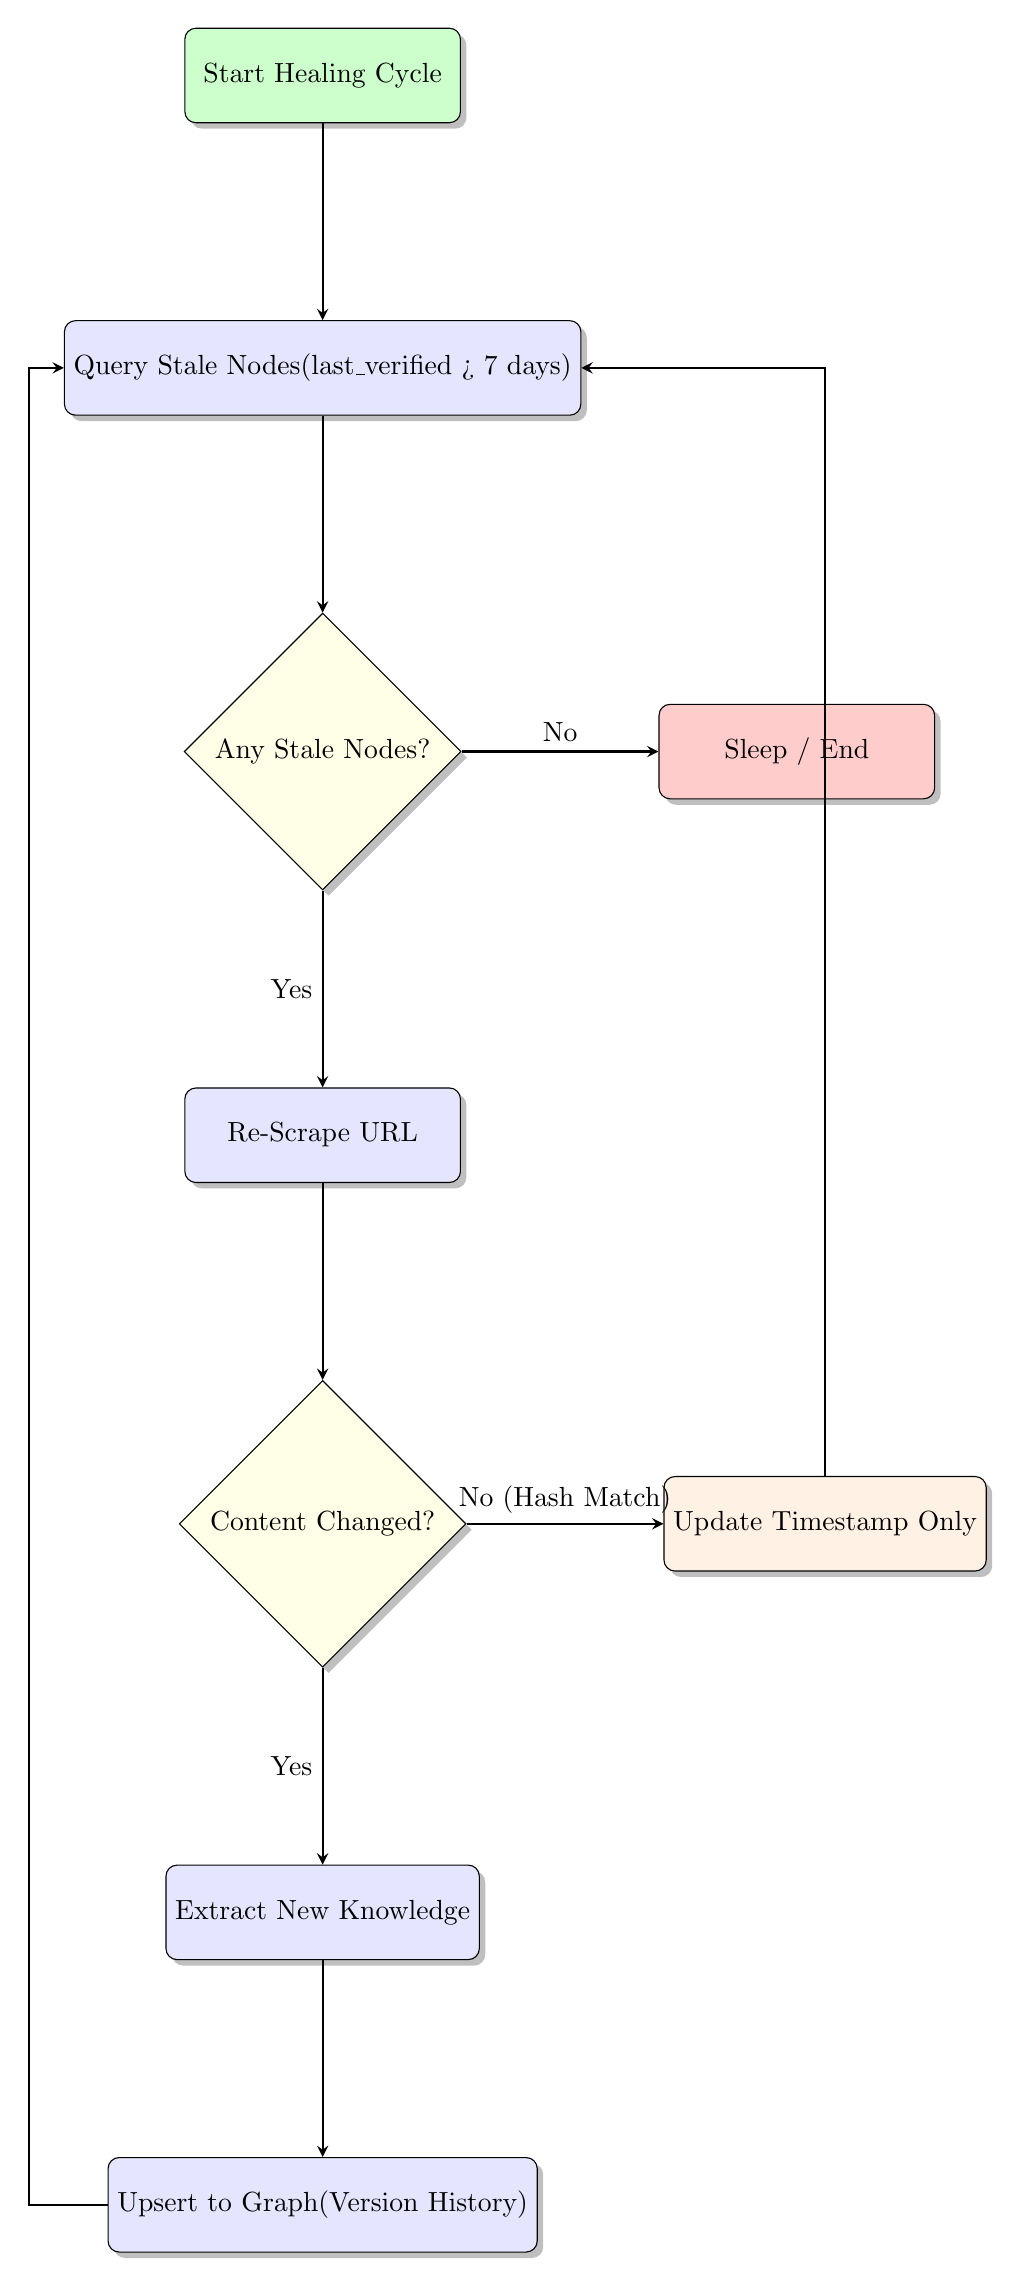
\begin{tikzpicture}[
    node distance=2.5cm,
    process/.style={rectangle, minimum width=3.5cm, minimum height=1.2cm, text centered, draw=black, fill=blue!10, drop shadow, rounded corners},
    decision/.style={diamond, minimum width=3cm, minimum height=1cm, text centered, draw=black, fill=yellow!10, drop shadow},
    arrow/.style={thick,->,>=stealth},
    line/.style={thick}
]

% Nodes
\node (start) [process, fill=green!20] {Start Healing Cycle};
\node (query) [process, below=of start] {Query Stale Nodes\\(last\_verified > 7 days)};
\node (check) [decision, below=of query] {Any Stale Nodes?};
\node (end) [process, right=of check, fill=red!20] {Sleep / End};

\node (scrape) [process, below=of check] {Re-Scrape URL};
\node (hash) [decision, below=of scrape] {Content Changed?};

\node (update_ts) [process, right=of hash, fill=orange!10] {Update Timestamp Only};
\node (extract) [process, below=of hash] {Extract New Knowledge};
\node (upsert) [process, below=of extract] {Upsert to Graph\\(Version History)};

% Edges
\draw [arrow] (start) -- (query);
\draw [arrow] (query) -- (check);
\draw [arrow] (check) -- node[anchor=south] {No} (end);
\draw [arrow] (check) -- node[anchor=east] {Yes} (scrape);

\draw [arrow] (scrape) -- (hash);
\draw [arrow] (hash) -- node[anchor=south] {No (Hash Match)} (update_ts);
\draw [arrow] (hash) -- node[anchor=east] {Yes} (extract);

\draw [arrow] (extract) -- (upsert);

% Loops
\draw [arrow] (update_ts) |- (query);
\draw [arrow] (upsert.west) -- ++(-1,0) |- (query.west);

\end{tikzpicture}
\end{document}
